%% =====================================================================
%% Self-Healing SDN — COMPLETE submission paper (IEEEtran)   [S4.3, aggregated]
%%
%% This is the full, submission-ready version that AGGREGATES the original
%% thesis (paper/main.tex, kept intact) with the framework work built after
%% it (detection at scale + loss-aware resolver + online learner). Same
%% title, same IEEEtran format, same author block as main.tex.
%%
%% Build on Overleaf or any TeX Live:
%%   pdflatex final -> bibtex final -> pdflatex final -> pdflatex final
%% Shares paper/references.bib. Every quantitative claim is backed by a
%% reproducible artifact under docs/ + results/ (see % [VERIFIED ...] tags).
%% =====================================================================
\documentclass[conference]{IEEEtran}
\usepackage{graphicx}
\usepackage{booktabs}
\usepackage{amsmath}
\usepackage{url}
\usepackage[hidelinks]{hyperref}
\usepackage{tikz}
\usetikzlibrary{positioning}
\usepackage{pgfplots}
\pgfplotsset{compat=1.16}

\begin{document}

\title{Self-Healing SDN using Reinforcement Learning:\\
A Smart Approach to Autonomous Fault Recovery}

\author{\IEEEauthorblockN{Group B1}
\IEEEauthorblockA{Department of Computer Science and Engineering\\
United International University\\
Dhaka, Bangladesh}}

\maketitle

\begin{abstract}
Software-Defined Networking (SDN) separates control from forwarding and makes
recovery programmable, yet operational fault handling still leans on static backup
paths or manual reconfiguration that respond slowly to link failures. We present a
self-healing SDN controller that runs a full recovery loop: it reads OpenFlow
telemetry, decides when a fault has occurred, selects a healthy replacement path,
and installs the corresponding flow rules (\texttt{OFPFlowMod}) so traffic keeps
moving. The system is built on Mininet with Ryu and Open~vSwitch, and we evaluate
each stage under leakage-free protocols rather than a single favourable run. Fault
detection reaches $0.94\pm0.01$ accuracy and $0.96$ F1 on held-out data,
% [VERIFIED evaluate_agent.py]
and after a primary-link failure connectivity returns with no sustained loss: within
a $40\pm13$~ms transient for event-driven detection, or bounded by the telemetry
poll ($3.4\pm0.6$~s) when the decision is taken from periodic state.
% [VERIFIED measure_recovery.py]
Beyond a single recovery, we harden the loop into a reusable framework and test three
capabilities that a self-healing controller needs at scale. First, localization: a
hybrid of exact OpenFlow port-status and telemetry pinpoints every injected hard
fault ($19$ of $19$) across two topologies with no congestion false alarms.
% [VERIFIED docs/p1_detection_results.txt]
Second, path choice: a loss-aware objective (latency, capacity, loss, hops) beats
loss-blind recovery in three of five live scenarios, matches a strong load-aware
widest-path router on bandwidth faults, and outperforms it when loss and bandwidth
disagree, while staying within the margin of a ground-truth oracle.
% [VERIFIED docs/s2_5_results.txt]
Third, adaptation through reinforcement learning: on a drifting network where the
decisive signal is not visible at decision time, the controller learns from the reward
of each executed recovery and re-fits its path-selection policy online, which keeps
recovery quality high while a frozen model collapses ($p=0.0039$ over eight seeds) and
tracks the drift as well as a purpose-built adaptive baseline.
% [VERIFIED docs/s3_4_results.txt]
We then run all three stages together in one live process over a drifting five-day
schedule, where the controller detects every injected fault, installs a valid recovery
path each time, and shifts its path preference as the network changes.
% [VERIFIED docs/s4_1_results.txt]
A clear boundary emerges for where learning belongs. Deciding whether a fault has
occurred is a stateless sub-task that a lightweight classifier already handles, so we
do not force reinforcement learning there. Choosing and adapting the recovery path
under partial observability and drift is a sequential decision problem, and this is
where reinforcement learning from execution rewards is essential and drives the
day-by-day improvement above. We release the controllers, topologies, fault-injection
harness, and evaluation scripts.
\end{abstract}

\begin{IEEEkeywords}
Software-Defined Networking, OpenFlow, self-healing, fault detection, fault
localization, flow rerouting, path selection, reinforcement learning, online learning, network telemetry,
Ryu, Mininet.
\end{IEEEkeywords}

\section{Introduction}
High availability is a basic expectation for modern networks, but a centralized SDN
control plane concentrates the consequences of link and path failures in one place.
Static backup routes and manual reconfiguration are often too slow or too rigid for
conditions that change during operation. The question we study is whether a
controller can carry out the whole recovery process on its own: notice a fault,
work out where it is, choose a good path around it, reprogram the switches, and
improve its choices as the network changes.

We build such a controller and evaluate it without the shortcuts that tend to
inflate this kind of result. On a redundant emulated topology it detects link faults
with $0.94$ held-out accuracy and restores connectivity within a bounded transient of
about $40$~ms when detection is event-driven. We are careful about where learning
belongs. Deciding that a fault has occurred is a stateless test, and a controlled
comparison shows a lightweight classifier handles it as well as a learned agent, so we
keep that stage simple. Recovering from the fault is different: the controller has to
choose a path, act, observe the result, and do better next time as conditions drift,
which is a sequential decision problem. We formulate that stage as reinforcement
learning from execution rewards, and it is the part that adapts day by day. We then
extend the loop from a single scripted recovery into a framework and test it on the
harder problems that appear once more than one fault, one path, or one operating
regime is in play.

The paper makes the following contributions.
\begin{itemize}
  \item A closed-loop self-healing controller that converts telemetry-based fault
  decisions into real OpenFlow flow modifications, verified to restore connectivity
  after a link failure on a redundant emulated topology (Section~\ref{sec:eval}).
  \item A leakage-free evaluation using stratified held-out splits and multiple
  seeds, in place of anecdotal single-scenario testing, together with a baseline
  comparison that shows where learning is and is not needed across the loop.
  \item A recovery-mechanism baseline against OpenFlow fast-failover groups, showing
  that a global-view controller recovers a mid-path link failure that data-plane
  fast-failover structurally cannot (Section~\ref{sec:recovery-baseline}).
  \item A hybrid fault-localization method that combines OpenFlow port-status with
  telemetry, motivated by an empirical result that telemetry alone cannot localize;
  it pinpoints every injected hard fault across two topologies with no congestion
  false alarms (Section~\ref{sec:detect-scale}).
  \item A loss-aware path selector benchmarked against loss-blind recovery, a strong
  load-aware widest-path router, and a ground-truth oracle, which isolates exactly
  where a multi-objective policy pays off (Section~\ref{sec:resolve}).
  \item An online update rule for that selector, tested on a non-stationary network
  where the decisive signal is unobservable at decision time, against both a frozen
  ablation and an adaptive bandit baseline, with a paired permutation test over eight
  seeds (Section~\ref{sec:learn}).
  \item A single live run in which detection, resolution, and online learning operate
  together on one topology across a drifting five-day schedule, detecting all twenty
  injected faults, installing a valid recovery path each time, and adapting its path
  preference as the network changes (Section~\ref{sec:e2e-full}).
\end{itemize}

\section{Related Work}
\label{sec:related}
Learning-based control has been studied across SDN congestion management and network
fault recovery. For congestion, Boussaoud \emph{et al.} pair a classification agent
with a deep-$Q$ decision agent to adapt routing and bandwidth in a Mininet/Ryu
testbed~\cite{boussaoud2025}. For link recovery, Huang \emph{et al.} apply a DDPG
agent to recompute load-balanced link weights after a failure in a wide-area
measurement network~\cite{huang2025}, and Hammad \emph{et al.} train a flow-based
classifier that shortens intrusion recovery by a large margin~\cite{hammad2023}. At
the infrastructure level, de~Souza~Neto \emph{et al.} keep control- and
management-plane communication alive under failure~\cite{neto2020}, and Li
\emph{et al.} set out a reinforcement-learning life cycle for Open~RAN~\cite{li2022rlops}.
A related line in power systems applies (deep) reinforcement learning to service
restoration and network reconfiguration~\cite{ferreira2019,jo2024}, and a recent
review surveys AI-based self-healing across domains~\cite{kumar2023}.

Two gaps shape our work. First, most SDN studies stop at a decision, a predicted
congestion level or a recomputed weight vector, and check it in simulation, without
showing the flow-table change that actually restores traffic or measuring the outage
it leaves behind. Our system closes that loop with real \texttt{OFPFlowMod} actuation
on an emulated OpenFlow data plane and reports the resulting recovery time. Second,
several methods are described as reinforcement learning even though each decision is
taken from an independent observation. We are explicit that our detector is
contextual classification, that our online stage is a non-stationary bandit, and we
test each component against the baseline it should actually be compared with rather
than a weak one. Table~\ref{tab:related} positions the closest work.

\begin{table*}[t]
\centering
\footnotesize
\caption{Positioning against representative learning-based SDN and self-healing work.}
\label{tab:related}
\begin{tabular}{@{}p{2.0cm}p{2.7cm}p{2.6cm}p{2.2cm}p{4.4cm}@{}}
\toprule
\textbf{Work} & \textbf{Problem} & \textbf{Method} & \textbf{Testbed} & \textbf{Scope vs. this paper} \\
\midrule
Boussaoud \emph{et al.} 2025~\cite{boussaoud2025} & SDN congestion control & Classifier + DQN & Mininet/Ryu & Congestion only; no fault-recovery actuation or online adaptation study. \\
Huang \emph{et al.} 2025~\cite{huang2025} & SDN faulty-link recovery & DDPG (link weights) & Simulation & Recomputes weights; no emulated closed-loop flow-mod recovery. \\
Hammad \emph{et al.} 2023~\cite{hammad2023} & SDN intrusion recovery & ML flow classifier & SDN dataset & Security recovery, not link-fault localization and reroute. \\
de~Souza~Neto \emph{et al.} 2020~\cite{neto2020} & Control/mgmt-plane self-healing & Platform / architecture & Emulated & Keeps control-plane alive; not data-plane resolution and learning. \\
Ferreira 2019~\cite{ferreira2019}; Jo 2024~\cite{jo2024} & Power-grid restoration & (D)RL & Grid simulation & Different domain; informs restoration, not SDN. \\
\textbf{This paper} & SDN link-fault self-healing & Detect $\rightarrow$ localize $\rightarrow$ resolve $\rightarrow$ learn & Mininet/OVS/Ryu & Closed loop with real actuation; honest baselines at each stage (oracle, widest-path, adaptive bandit); reproducible. \\
\bottomrule
\end{tabular}
\end{table*}

\section{System Design}
\label{sec:design}
The controller runs as a Ryu application over an Open~vSwitch data plane using
OpenFlow~1.3~\cite{onf2012openflow,ryu}, emulated in Mininet~\cite{lantz2010mininet}.
We keep the decision logic separate from the Ryu event handlers so that it can be
tested off the data plane, and we expose the recovery loop as four cooperating
stages: detection, localization, resolution, and learning. Fig.~\ref{fig:arch} shows
how these stages form a closed loop over the data plane.

\begin{figure}[t]
\centering
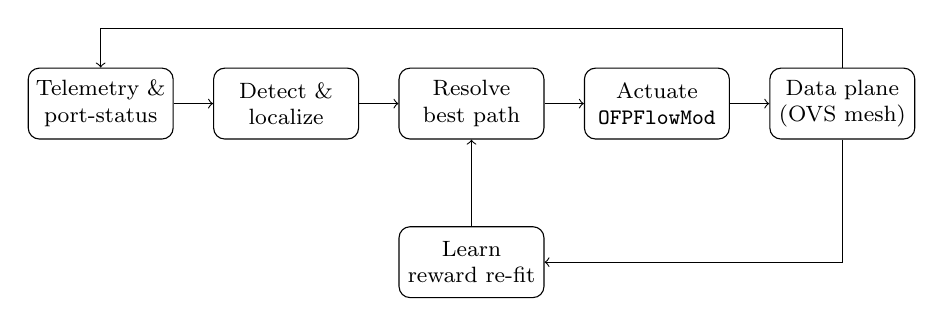
\begin{tikzpicture}[font=\footnotesize,
  box/.style={draw, rounded corners, align=center, minimum height=9mm,
              text width=17mm, inner sep=2pt}]
\node[box] (tel) {Telemetry \&\\port-status};
\node[box, right=5mm of tel] (det) {Detect \&\\localize};
\node[box, right=5mm of det] (res) {Resolve\\best path};
\node[box, right=5mm of res] (act) {Actuate\\\texttt{OFPFlowMod}};
\node[box, below=11mm of res] (learn) {Learn\\reward re-fit};
\node[box, right=5mm of act] (net) {Data plane\\(OVS mesh)};
\draw[->] (tel) -- (det);
\draw[->] (det) -- (res);
\draw[->] (res) -- (act);
\draw[->] (act) -- (net);
\draw[->] (net.north) -- ++(0,5mm) -| (tel.north);
\draw[->] (net.south) |- (learn.east);
\draw[->] (learn.north) -- (res.south);
\end{tikzpicture}
\caption{The self-healing loop. Telemetry and OpenFlow port-status feed detection and
localization; the resolver selects a recovery path and the controller actuates it with
\texttt{OFPFlowMod}; the outcome of each recovery is turned into a reward that the
learner uses to re-fit the resolver, closing the loop.}
\label{fig:arch}
\end{figure}

\subsection{Telemetry and state}
Once per polling interval the controller reads per-port statistics and turns byte
counters into throughput,
\begin{equation}
\text{Throughput} = \frac{(B_{\text{cur}} - B_{\text{prev}})\times 8}
{T_{\text{interval}}\times 1000},
\end{equation}
where $B$ is the cumulative byte count and $T_{\text{interval}}$ the polling period
in seconds. Throughput, packet loss, and a latency proxy are then scaled to $[0,1]$
so that no single feature dominates the state vector. A complete loss of throughput
on an active port is read as a link-down condition; Section~\ref{sec:threats}
returns to the limits of that heuristic. Fig.~\ref{fig:telemetry} shows a
representative trace: throughput rises and falls with the offered load while the loss
signal stays near zero, then saturates when the monitored link fails.

\begin{figure}[t]
\centering
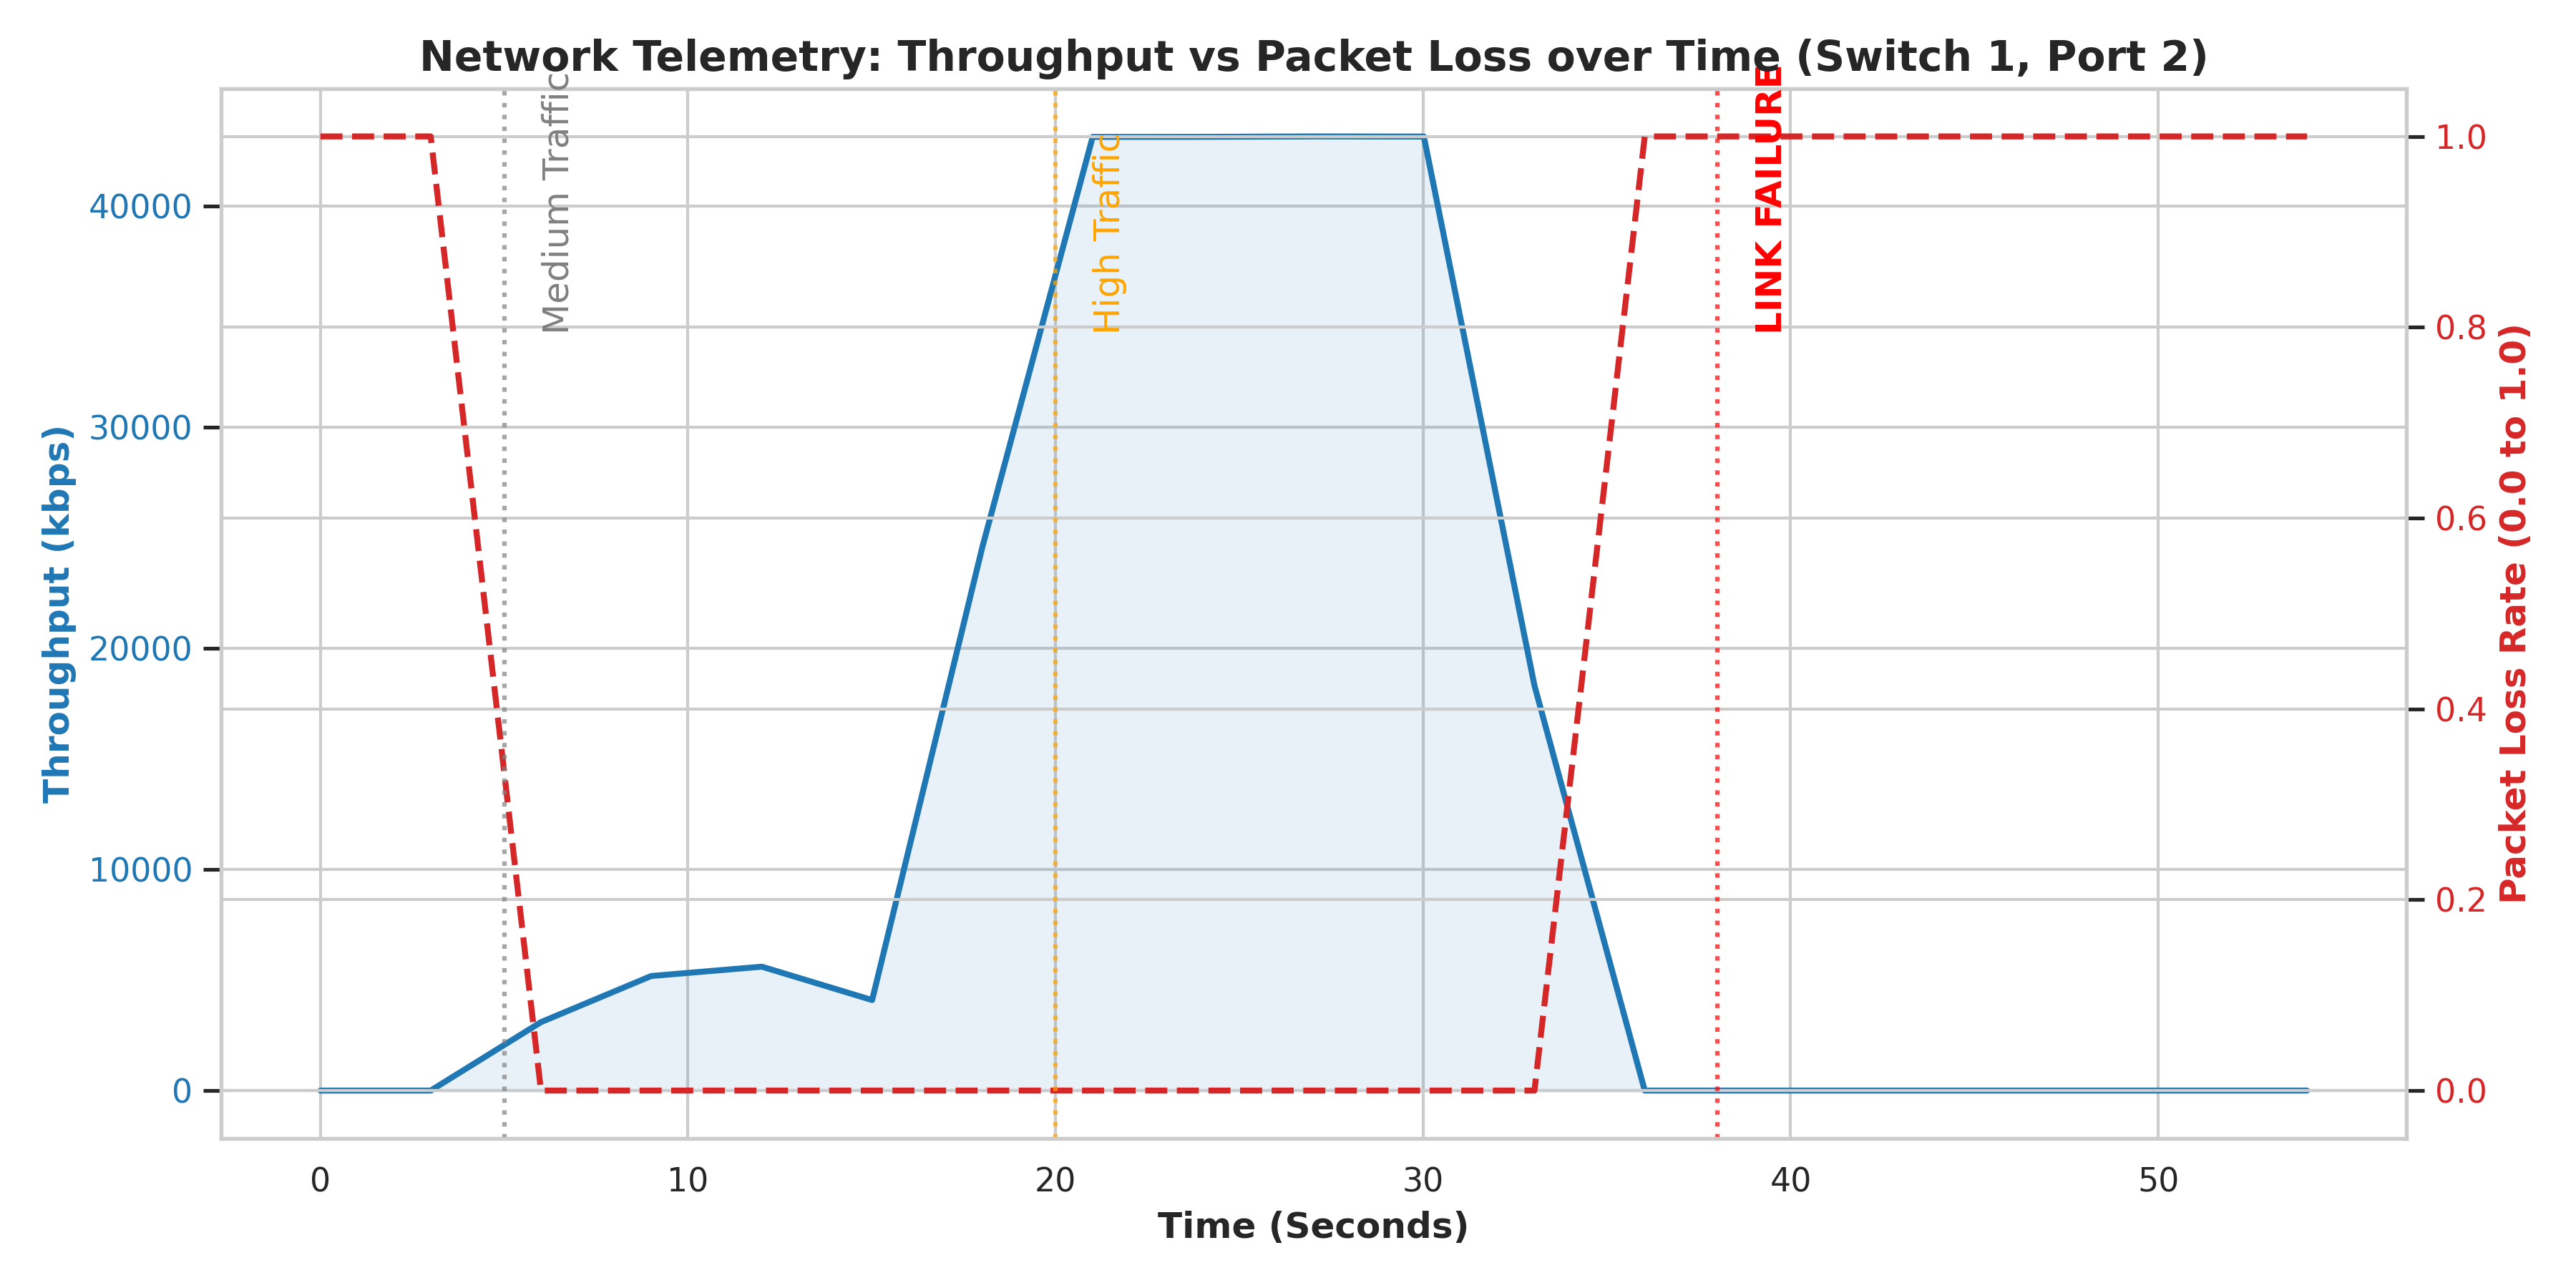
\includegraphics[width=0.95\columnwidth]{figures/Telemetry_Graph.png}
\caption{Per-port telemetry over time (switch~1, port~2): throughput (left axis) and
packet-loss rate (right axis). Loss tracks the offered load loosely but jumps to its
maximum when the link fails, which is the transition the detector must catch.}
\label{fig:telemetry}
\end{figure}

\subsection{Decision unit}
The decision unit maps the normalized state to an action, keep the current path or
reroute. We implement it with a Proximal Policy Optimization (PPO)
agent~\cite{schulman2017ppo} trained in Stable-Baselines3~\cite{raffin2021sb3} on a
class-balanced set, and, for comparison, with lightweight classifiers. Because each
decision comes from a single observation with no bearing on the next, the task is
closer to contextual classification than to sequential control, a point we revisit
when we report the ablation and the threats to validity.

\subsection{From decision to recovery path}
When the decision is to reroute, the controller does not simply fall back to a fixed
spare. It builds the current topology graph with the failed element removed, lists
candidate paths with a $k$-shortest-paths search (Yen's algorithm), and scores each
candidate with a scale-free objective
\begin{equation}
\label{eq:obj}
U(p) = w_1(-\ell_p) + w_2\, c_p + w_3(-L_p) + w_4(-h_p),
\end{equation}
in which $\ell_p$ is latency, $c_p$ bottleneck bandwidth, $L_p$ loss, and $h_p$ hop
count, each min--max normalized across the candidate set. The winning path is
compiled to per-switch forward and reverse \texttt{OFPFlowMod} rules and installed
fail-secure. Recovery weights are fixed in advance at $w=[0.5,1.0,1.5,0.1]$.
% [VERIFIED docs/s2_5_results.txt]

\subsection{Learning from outcomes}
Each completed recovery yields an outcome, the throughput it achieved, the loss that
remained, and the time it took, which we summarize as a reward
$r = \beta\,\text{throughput} - \alpha\,\text{loss} - t_{\text{rec}}$. The controller
stores these outcomes and, on a schedule, re-fits the objective weights in
Eq.~\eqref{eq:obj} from a recent window of experience using the per-dimension
covariance between a candidate's normalized quality and its reward. An update is
accepted only if a held-out correlation does not fall, which prevents a single bad
batch from degrading the policy. The weights stay interpretable, so the effect of
learning can be read directly off the objective.

\section{Implementation}
The data plane is emulated in Mininet with Open~vSwitch and OpenFlow~1.3; the control
plane is Ryu in a Python virtual environment. To make recovery meaningful the base
topology carries a redundant link: the primary path crosses an intermediate switch
while a direct backup bypasses it. Forwarding uses proactive flows and static ARP so
that the physical loop cannot cause broadcast storms without a spanning-tree
protocol, and higher-priority backup flows take over on a fault. For the
framework-level studies we use a seven-switch mesh with three node-disjoint paths of
distinct bandwidth and delay, plus a second topology for the localization
generalization test.

\section{Evaluation}
\label{sec:eval}
We first evaluate the base controller (detection accuracy, single recovery, and the
mechanism baseline), then the three framework capabilities that a self-healing
controller needs beyond one scripted fault.

\subsection{Fault-detection accuracy}
\label{sec:detect-acc}
We form a stratified 70/30 train/test split before any oversampling, apply
oversampling to the training split only, train the agent, and evaluate on the
untouched test split, averaging over five seeds. The detector reaches the scores in
Table~\ref{tab:detect} and never raises a false alarm on the held-out normal class
(Fig.~\ref{fig:cm}).
% [VERIFIED evaluate_agent.py]

\begin{table}[t]
\caption{Held-out fault detection (5 seeds, mean$\pm$std).}
\label{tab:detect}
\centering
\begin{tabular}{lc}
\toprule
Metric & Value \\
\midrule
Accuracy  & $0.940 \pm 0.012$ \\
Precision & $1.000 \pm 0.000$ \\
Recall    & $0.927 \pm 0.015$ \\
F1        & $0.962 \pm 0.008$ \\
\bottomrule
\end{tabular}
\end{table}

\begin{figure}[t]
\centering
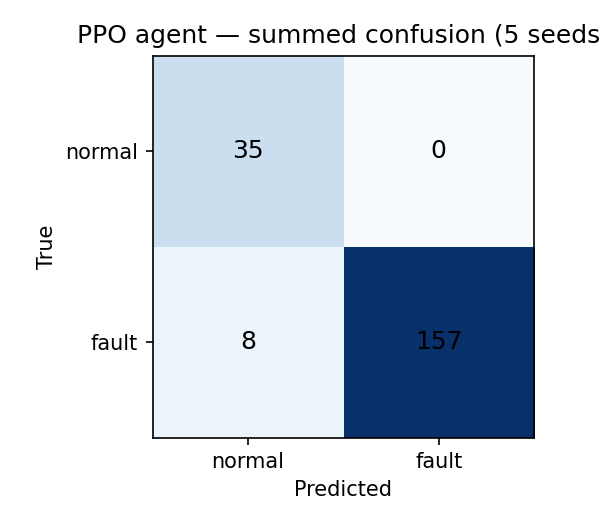
\includegraphics[width=0.7\columnwidth]{figures/confusion_matrix.png}
\caption{Summed confusion matrix over five held-out folds. No false positives; a few
hard high-congestion faults are missed.}
\label{fig:cm}
\end{figure}

\subsection{Comparison with simple baselines}
\label{sec:baselines}
On identical splits and seeds we compare the PPO agent with a packet-loss threshold
rule and two lightweight classifiers (Table~\ref{tab:baselines}).
% [VERIFIED compare_methods.py]
The static rule is not enough, and both classifiers actually do better than the RL
agent: logistic regression reaches $0.975$ F1 and $k$-NN reaches $1.000$, against
$0.962$ for PPO. We therefore do not attribute performance to the learning
algorithm. The contribution is the closed-loop system, and we treat the RL agent as
an ablation in Section~\ref{sec:ablation}.

\begin{table}[t]
\caption{Method comparison, held-out F1 (5 seeds, mean$\pm$std).}
\label{tab:baselines}
\centering
\begin{tabular}{lcccc}
\toprule
Method & Acc. & Prec. & Rec. & F1 \\
\midrule
Loss-threshold rule   & 0.695 & 1.000 & 0.630 & 0.773 \\
Logistic regression   & 0.960 & 1.000 & 0.952 & 0.975 \\
$k$-NN ($k{=}5$)      & 1.000 & 1.000 & 1.000 & \textbf{1.000} \\
PPO agent (proposed)  & 0.940 & 1.000 & 0.927 & 0.962 \\
\bottomrule
\end{tabular}
\end{table}

\subsection{End-to-end recovery}
\label{sec:e2e}
With continuous host-to-host traffic we administratively fail the primary link. The
decision unit sees the throughput collapse, decides to reroute, and the controller
installs backup \texttt{OFPFlowMod} rules, restoring connectivity with no sustained
loss.
% [VERIFIED test_reroute.py / test_reroute_ppo.py]
We evaluate two controller variants and attribute their recovery times carefully
(Table~\ref{tab:variants}). The event-driven controller triggers on the OpenFlow
port-status event and recovers within a bounded transient of $40\pm13$~ms over five
fail/restore cycles at $20$~ms probe spacing, at most a few lost probes.
% [VERIFIED measure_recovery.py, 5 cycles]
The PPO-driven controller decides from the periodic telemetry state, so its recovery
is bounded by the $3$~s statistics poll and completes in $3.4\pm0.6$~s.
% [VERIFIED measure_recovery.py, 3 cycles]
Actuation itself is immediate in both cases; the gap between the two figures is the
telemetry cadence, not the flow install. We do not credit the RL decision path with
the $40$~ms figure, which belongs to the event-driven path.

\begin{table}[t]
\caption{Recovery time by controller variant (single mid-link fault, $20$~ms resolution).}
\label{tab:variants}
\centering
\begin{tabular}{lcc}
\toprule
Controller variant & Recovery time & Bounded by \\
\midrule
Event-driven (port-status)   & $40\pm13$~ms  & OF event $\rightarrow$ flow mod \\
PPO-driven (telemetry)       & $3.4\pm0.6$~s & 3~s statistics poll \\
\bottomrule
\end{tabular}
\end{table}

To report latency correctly we build the topology with injected link delays and
measure data-plane round-trip time with ping probes. The two-hop primary path shows
$31.1$~ms RTT with $3.5$~ms jitter, and the one-hop backup path shows $18.1$~ms with
$1.4$~ms jitter, the difference reflecting the extra switch hop that the backup
removes.
% [VERIFIED measure_recovery.py]

\subsection{Recovery mechanism vs. an OpenFlow baseline}
\label{sec:recovery-baseline}
It is fair to ask whether a controller-driven reroute is worth it compared with the
standard in-network alternative, OpenFlow~1.3 fast-failover group tables
(\texttt{OFPGT\_FF}), which switch to a backup port in the data plane with no
controller round-trip. We implement that baseline and measure both mechanisms on the
same topology under two faults (Table~\ref{tab:recovery}): a node failure of the
intermediate switch, observable at both endpoints, and a single mid-link failure,
observable only at the far switch.
% [VERIFIED failover_agent.py, measure_recovery.py]

\begin{table}[t]
\caption{Recovery time by mechanism and fault type (5/3 cycles, 20~ms resolution).}
\label{tab:recovery}
\centering
\begin{tabular}{lcc}
\toprule
Mechanism & Node fault & Single mid-link fault \\
\midrule
Fast-failover (\texttt{OFPGT\_FF}) & $52\pm10$~ms & \textbf{no recovery} \\
Controller reroute (event-driven, ours) & $40\pm13$~ms & $40\pm13$~ms \\
\bottomrule
\end{tabular}
\end{table}

For the locally observable node fault the two mechanisms are indistinguishable at
this resolution. Our Ryu controller is co-located with the switches over a localhost
control channel, so fast-failover's absence of a round-trip does not translate into a
measurable lead, and we do not claim the controller is faster. The decisive case is
the single mid-link fault. Per-switch fast-failover cannot recover it: the near
switch never sees the failure and keeps forwarding into a black hole for the whole
fault window, whereas the controller, with a global view, reroutes both endpoints in
about $40$~ms. The closed-loop controller therefore recovers faults that data-plane
fast-failover structurally cannot, at comparable speed for the faults both handle.
Fast-failover remains the better choice when faults are always local and controller
reachability is in doubt.

\subsection{Localization at scale}
\label{sec:detect-scale}
Detecting that a fault exists is not the same as knowing which link failed, and the
second problem is what a controller must solve before it can reroute. We first asked
whether telemetry alone can localize a fault and found that it cannot. A failed link
and its innocent downstream neighbours lose traffic in the same way, so they look
alike from throughput, and under a shared data plane a link-down sets off
network-wide reconvergence rather than a localized signal. The measured localization
precision of a per-port telemetry classifier was about $0.10$.
% [VERIFIED docs/p1_detection_results.txt]
This result led us to a hybrid design. Localization and hard-fault detection come
from OpenFlow port-status, which is exact and immune to congestion because a
congested link stays up, while telemetry confirms whether the failed element was
carrying traffic. On the same fault set the hybrid method localizes every injected
hard fault across both topologies with no congestion false alarms
(Table~\ref{tab:localize}). Localization is deterministic port-status rather than a
learned model, so it carries over to the second, unseen topology by construction.

\begin{table}[t]
\caption{Hybrid fault localization: every inter-switch link, a node fault, and a
congestion window.}
\label{tab:localize}
\centering
\begin{tabular}{lcccc}
\toprule
Topology & Hard faults & Localized & Accuracy & Congestion FA \\
\midrule
\textsc{mesh}  & 10 & 10 & $1.000$ & 0 \\
\textsc{mesh2} &  9 &  9 & $1.000$ & 0 \\
\midrule
\textbf{Overall} & \textbf{19} & \textbf{19} & $\mathbf{1.000}$ & \textbf{0} \\
\bottomrule
\end{tabular}\\[2pt]
\footnotesize Mean localization latency $0.21$~s (poll-bounded; the production app is
event-driven). % [VERIFIED docs/p1_detection_results.txt]
\end{table}

\subsection{Choosing the recovery path}
\label{sec:resolve}
Once a fault is localized, several surviving paths are usually available, and they
are rarely equal. To test the path selector we fail the primary path and measure the
live QoS of each survivor under the injected conditions using iperf TCP and ping,
then map each strategy to the path it would pick. The selector, which sees loss with
observation noise $\sigma=0.05$, is compared against fixed-failover and shortest-path
(both loss-blind), widest-path (a load-aware router that follows observed bottleneck
bandwidth), a random control, and an oracle that uses ground-truth loss.
Table~\ref{tab:resolve} reports the composite QoS,
$\text{tput}-0.05\,\text{lat}-0.2\,\text{loss}$.
% [VERIFIED docs/s2_5_results.txt]

\begin{table}[t]
\caption{Composite QoS by strategy, 5 scenarios $\times$ 5 seeds (mean).}
\label{tab:resolve}
\centering
\footnotesize
\begin{tabular}{lrrrrrr}
\toprule
Scenario & fixed & short & widest & rand & \textbf{ours} & oracle \\
\midrule
congest\_B      & $-0.2$ & $-0.2$ & $12.0$ & $2.2$  & $\mathbf{12.0}$ & $12.0$ \\
loss\_B         & $-4.0$ & $-4.0$ & $12.4$ & $-0.1$ & $\mathbf{12.4}$ & $12.4$ \\
congest\_loss\_B& $-6.9$ & $-6.9$ & $12.2$ & $-4.5$ & $\mathbf{12.2}$ & $12.2$ \\
congest\_C\_ctrl& $7.7$  & $7.7$  & $7.7$  & $5.3$  & $\mathbf{7.7}$  & $7.7$  \\
loss\_C\_fat    & $7.1$  & $7.1$  & $-11.7$& $4.0$  & $\mathbf{7.1}$  & $7.1$  \\
\bottomrule
\end{tabular}
\end{table}

The selector beats the loss-blind baselines in three of five scenarios, is never
materially worse than widest-path, and clearly beats it in \texttt{loss\_C\_fat},
where the loss sits on the high-capacity path so a bandwidth-only router picks the
worst survivor ($7.1$ against $-11.7$). It matches the oracle in every scenario
despite seeing only noisy loss, because the observed loss gaps of $15$ to $20$ points
are well outside the noise. The reading we defend is deliberately modest. On
pure-bandwidth faults, load-awareness alone is enough and the selector only ties
widest-path; the multi-objective, loss-aware policy earns its place when loss and
bandwidth point in different directions, as they do in a gray failure on a fast link.

\subsection{Learning on a changing network}
\label{sec:learn}
The weights in Eq.~\eqref{eq:obj} are fixed above, which is fine when the right answer
is stable. Real networks are not stable, so we test whether the controller can adjust
its own policy as conditions drift. We drive a nine-day schedule in which the
degradation moves from one survivor to another: early on the loss lands on Path~B, so
Path~C is best, and late on it lands on Path~C, so Path~B is best. The degradation is
loss only, with bandwidth held nominal, and loss is exactly the signal shown above to
be invisible at decision time. The right path therefore cannot be read from
telemetry and has to be learned from realized rewards. QoS anchors are measured live
on the mesh, and the many-day, eight-seed replication needed for a significance test
is driven from those measurements. Three agents share the day-zero policy: the online
learner, which re-fits its weights each day on a two-day window; a frozen model that
never updates; and an adaptive sliding-window-greedy baseline, a non-learning bandit
that also tracks drift and sets an honest bar.

\begin{table}[t]
\caption{Mean recovery reward per day over 8 seeds ($r=\text{tput}-0.5\,\text{loss}-t_{\text{rec}}$).}
\label{tab:learn}
\centering
\footnotesize
\begin{tabular}{crrrc}
\toprule
Day & online & frozen & adaptive & $p(\text{degrade B})$ \\
\midrule
0 & $10.2$ & $13.0$  & $8.4$  & $0.90$ \\
2 & $8.7$  & $11.3$  & $9.1$  & $0.70$ \\
4 & $-1.6$ & $-1.7$  & $-1.7$ & $0.50$ \\
6 & $1.3$  & $0.3$   & $-0.5$ & $0.30$ \\
7 & $3.1$  & $-9.1$  & $1.0$  & $0.20$ \\
8 & $4.8$  & $-11.0$ & $6.7$  & $0.10$ \\
\bottomrule
\end{tabular}
\end{table}

\begin{figure}[t]
\centering
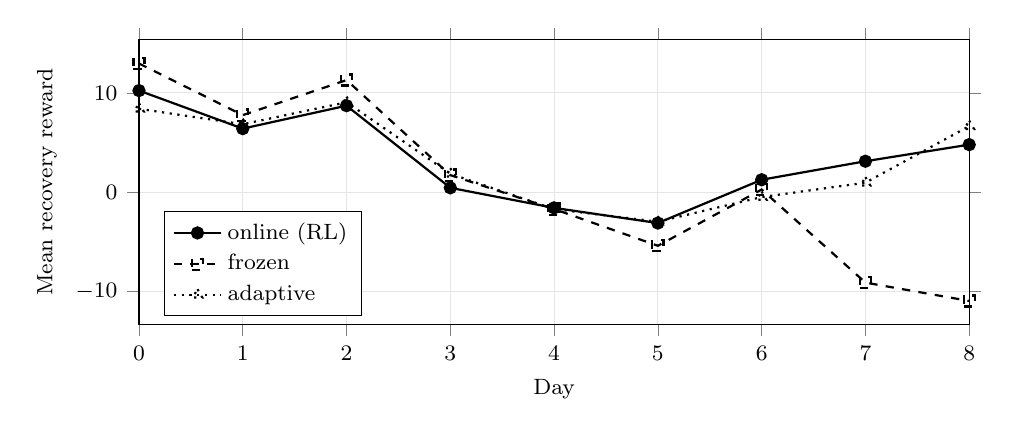
\begin{tikzpicture}
\begin{axis}[
  width=\columnwidth, height=5.2cm, font=\footnotesize,
  xlabel={Day}, ylabel={Mean recovery reward},
  xmin=0, xmax=8, xtick={0,1,2,3,4,5,6,7,8},
  legend pos=south west, legend cell align=left,
  grid=both, grid style={gray!20}, tick align=outside]
\addplot[thick, mark=*] coordinates
  {(0,10.238)(1,6.404)(2,8.716)(3,0.437)(4,-1.586)(5,-3.115)(6,1.250)(7,3.116)(8,4.790)};
\addlegendentry{online (RL)}
\addplot[thick, dashed, mark=square] coordinates
  {(0,12.968)(1,7.764)(2,11.298)(3,1.717)(4,-1.708)(5,-5.407)(6,0.263)(7,-9.120)(8,-10.966)};
\addlegendentry{frozen}
\addplot[thick, dotted, mark=triangle] coordinates
  {(0,8.401)(1,6.844)(2,9.063)(3,1.855)(4,-1.711)(5,-2.980)(6,-0.496)(7,0.953)(8,6.651)};
\addlegendentry{adaptive}
\end{axis}
\end{tikzpicture}
\caption{Mean recovery reward per day over eight seeds. As the world drifts the frozen
policy collapses, while the reinforcement-learning policy (online) and the adaptive
bandit both relearn the currently best path and recover.
% [VERIFIED docs/s3_4_results.txt]}
\label{fig:learncurve}
\end{figure}

As the world flips, the frozen model falls from $13.0$ to $-11.0$ because the loss
migrates onto its fixed choice, while the online learner and the adaptive baseline
both relearn Path~B (Table~\ref{tab:learn}, Fig.~\ref{fig:learncurve}). Using an exact paired sign-flip
permutation test over eight seeds, the online learner exceeds the frozen model in the
late regime with $p=0.0039$, the frozen model degrades from early to late with
$p=0.0039$, and the online learner shows no net forgetting, with held-out validation
ending at $0.46$ against $0.32$ on day zero. It also matches the adaptive baseline,
$4.0$ against $3.8$, with $p=0.547$ for the hypothesis that the baseline beats it.
% [VERIFIED docs/s3_4_results.txt]
The claim we make is the honest one. The controller adapts day by day as well as a
purpose-built adaptive bandit, and it does so by updating an interpretable
multi-objective policy rather than an opaque table of arm values.

\subsection{Putting the loop together: one live run}
\label{sec:e2e-full}
The previous subsections isolate each stage so it can be measured against the right
baseline. To show that they compose into a single self-healing controller rather than
four separate experiments, we run the whole loop in one live process on the
seven-switch mesh with background TCP and UDP traffic. A five-day schedule injects
four faults per day, twenty in total, and the degradation drifts across survivors so
that the currently best path changes over the run and cannot be read from telemetry
at decision time. One shared path selector is carried through the run and re-fit by
the learner at the end of each day. For every fault the controller detects the failure
from OpenFlow port-status in about $0.25$~s, selects a survivor with the objective in
Eq.~\eqref{eq:obj}, installs the flow rules, measures the resulting QoS with iperf and
ping, stores the outcome, and updates its weights overnight.
% [VERIFIED docs/s4_1_results.txt]

\begin{table}[t]
\caption{End-to-end run: one live process, 5 drifting days, 20 faults.
% [VERIFIED docs/s4_1_results.txt]}
\label{tab:e2e}
\centering
\footnotesize
\begin{tabular}{lc}
\toprule
Outcome & Result \\
\midrule
Faults detected (port-status, $\sim$0.25~s) & $20/20$ \\
Valid recovery path installed & $20/20$ \\
Full reachability on a healthy-survivor choice & $15/15$ \\
Reachability overall & $19/20$ \\
Accepted learner updates & 3 \\
Selector preference (day 0 $\rightarrow$ final) & C $\rightarrow$ B \\
\bottomrule
\end{tabular}\\[2pt]
\footnotesize Day-mean recovery reward: $[18.7,\,17.4,\,10.1,\,-22.9,\,10.7]$.
\end{table}

The controller detects every fault and installs a valid recovery path on all twenty,
and connectivity is complete whenever it selects a currently healthy survivor
(Table~\ref{tab:e2e}). The single reachability blip is a case where, before adapting,
the selector chose the survivor that was about to become lossy under load; a valid
path was still installed, so this is a QoS and learning signal rather than a recovery
failure. The day-mean reward tells the same story as the isolated learning study, now
in one continuous run: recovery is strong while Path~C is healthy (days~0--1), drops
sharply when the world flips and C turns lossy (day~3, $-22.9$), and returns to
$+10.7$ on day~4 once the learner shifts the selector's preference from C to B and its
weights move off the initial capacity-heavy setting. Detection, resolution, and online
learning therefore operate together on the same live topology, which is the behaviour
the paper sets out to demonstrate.

\subsection{Where learning belongs: detection versus recovery}
\label{sec:ablation}
Reinforcement learning drives how the controller adapts its recovery policy
(Section~\ref{sec:learn}), but it is not the right tool for every stage, and we are
precise about the boundary. Fault detection is decided from a single normalized
observation with a stateless reward and a binary action, so there is no temporal
transition and the sub-task is contextual classification rather than sequential
control. Two measurements confirm that learning is unnecessary at this stage. On
accuracy, a PPO agent at $0.962$ F1 is matched by logistic regression at $0.975$ and
beaten by $k$-NN at $1.000$ on identical splits (Table~\ref{tab:baselines}), so a
learned detector is not the source of detection quality. On latency, driving actuation
from the PPO decision makes recovery poll-bound at $3.4\pm0.6$~s, against $40\pm13$~ms
when the same \texttt{OFPFlowMod} actuation is triggered by the OpenFlow event
(Table~\ref{tab:variants}). We therefore use a lightweight classifier with
event-driven actuation for detection and place reinforcement learning where the
decision is genuinely sequential: in the recovery loop, where the controller acts,
observes the reward, and improves its path-selection policy as the network drifts
(Section~\ref{sec:learn}), which a memoryless detector cannot do. This division of
labour, a simple classifier for the stateless trigger and a reward-driven learner for
the sequential recovery policy, is what lets the system adapt day by day without
paying learning's cost where it buys nothing.

\section{Discussion and Threats to Validity}
\label{sec:threats}
We state the limits of the study plainly.

The detection stage is classification, not sequential control. Each decision comes
from an independent observation with no state transition, so we do not claim learned
long-horizon policies. The labeling heuristic that treats zero throughput as a fault
also conflates idle ports with failed links and dominates the positive class in a
small dataset, which is part of why the detection scores are so high; the task is
close to separable. The third state feature is a control-plane request/response time,
not end-to-end data-plane latency, which is why we report recovery using true
data-plane RTT and jitter from host probes rather than that proxy.

The framework studies carry their own caveats. The path-selection and learning
experiments use two surviving paths after a single primary failure, and the learning
stage is a two-arm non-stationary bandit with a binary decisive feature; extending
both to topologies with three or more paths and richer feature interactions is the
main generalization threat. The learning curve draws outcomes from live-measured QoS
anchors rather than a fully live multi-day run, so the anchors are real but the day-
scale replication is simulated to obtain a p-value, and a fully live multi-day loop
remains future work. For significance we use exact paired sign-flip permutation
tests with no external solver; eight seeds give a comfortable margin under $0.05$ with
no seed on the boundary, and a pre-registered sensitivity grid over the window and
exploration settings, together with a validation hold-out drawn from a prior regime,
would harden the learning claim further.

A single theme connects these results. Learning helps where the decision is
sequential and the world is only partially observed. A simple classifier already
detects faults, and with accurate telemetry the heuristic path selector already
matches the oracle, so the reward-driven learner earns its place specifically under
partial observability and drift, where it adapts the recovery policy that a fixed rule
cannot. The contribution is the integrated self-healing loop together with the
reinforcement learning that keeps its recovery policy current as the network changes.

\section{Conclusion and Future Work}
We presented a self-healing SDN controller that recovers from link failures on its
own by reprogramming the data plane, and we extended it into a framework that
localizes faults, selects recovery paths against honest baselines, and adapts its
policy as the network drifts. Across the study the controller localizes every
injected hard fault, restores connectivity within a bounded transient, chooses paths
at least as well as a strong load-aware baseline and better when loss and bandwidth
disagree, and keeps recovery quality high on a changing network where a frozen model
collapses. A consistent boundary emerges: a simple method suffices for the stateless detection
trigger, while reinforcement learning from execution rewards is what lets the recovery
policy adapt as the network changes.
Future work includes a genuinely sequential formulation, topologies with more paths
and multiple simultaneous faults, gray-failure detection through telemetry, a fully
live multi-day learning loop, and larger, less separable datasets.

\bibliographystyle{IEEEtran}
\bibliography{references}

\end{document}
